\begin{figure}[htbp]
\centering
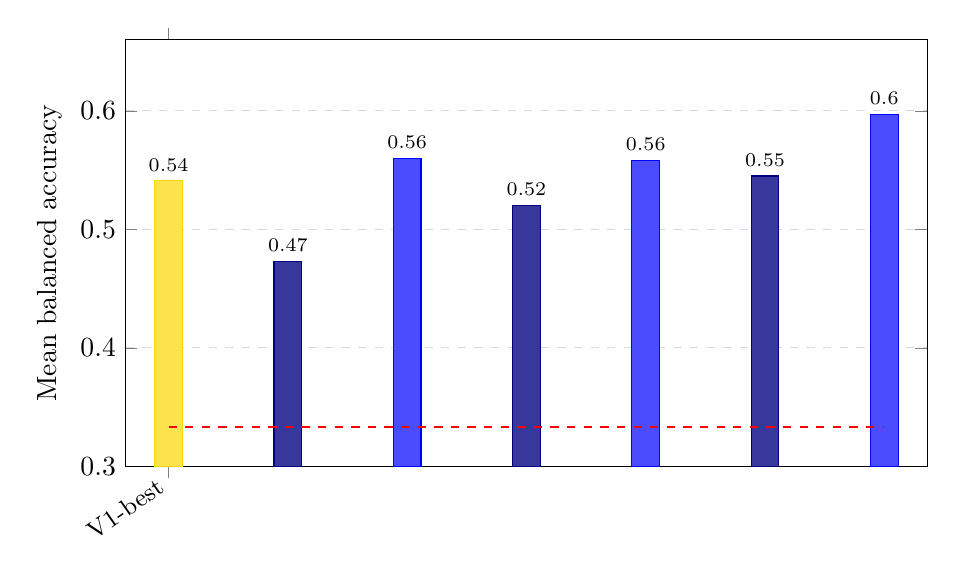
\begin{tikzpicture}
\begin{axis}[
  ybar,
  bar shift=0pt,
  width=0.97\textwidth,
  height=70mm,
  ymin=0.30,ymax=0.66,
  ylabel={Mean balanced accuracy},
  symbolic x coords={V1-best,V2-primary,V2-Tucker,V3-primary,V3-spectral,V4-primary,V4-SVM},
  xtick=data,
  x tick label style={rotate=35,anchor=east,font=\small},
  ymajorgrids=true,
  grid style={dashed,gray!30},
  nodes near coords,
  every node near coord/.append style={font=\scriptsize},
  enlarge x limits=0.06
]
\addplot[fill=Gold!70,draw=Gold] coordinates {(V1-best,0.541)};
\addplot[fill=Navy!78,draw=Navy] coordinates {(V2-primary,0.473) (V3-primary,0.520) (V4-primary,0.545)};
\addplot[fill=Blue!70,draw=Blue] coordinates {(V2-Tucker,0.560) (V3-spectral,0.558) (V4-SVM,0.597)};
\draw[dashed,thick,Red] (axis cs:V1-best,0.333) -- (axis cs:V4-SVM,0.333);
\end{axis}
\end{tikzpicture}
\caption{Experiment progression. Navy bars are predeclared complete-pipeline endpoints; blue bars are secondary best-family results; the V1 maximum is exploratory. The dashed baseline is 33.3\% balanced accuracy.}
\label{fig:experiment-evolution}
\end{figure}
